\documentclass[12pt,a4paper]{article}
\usepackage[utf8]{inputenc}
\usepackage{amsmath}
\usepackage{amsfonts}
\usepackage{amssymb}
\usepackage{enumerate}
%bold Greek letters and other symbols
\usepackage{bm}
\usepackage{graphics}
\usepackage[T1]{fontenc}
\usepackage[english]{babel}
\usepackage{graphicx}
\usepackage[left=2.5cm,right=3.0cm,top=2.5cm,bottom=3cm]{geometry}
\usepackage{color}
%
\usepackage{makeidx}
\usepackage{shortvrb,latexsym}

\setlength{\parindent}{0pt}
%\renewcommand{\floatpagefraction}{.99}
%\renewcommand{\textfraction}{.01}
\def \AA  {\bm{A}}
\def \uu  {\bm{u}}
\def \oo {\bm{\omega}}
\def \curl {\bm{\nabla}\times}
\def \dive {\bm{\nabla}\cdot}
\def \AA  {\bm{A}}
\newcommand{\bu}{\bm{u}}
\newcommand{\bv}{\bm{v}}
\newcommand{\br}{\bm{r}}
\newcommand{\rd}{\mathrm{d}}
\newcommand{\hx}{{\bf\hat{x}}}
\newcommand{\hy}{{\bf\hat{y}}}
\newcommand{\hz}{{\bf\hat{z}}}
\newcommand{\hr}{{\bf\hat{r}}}
\newcommand{\hn}{{\bf\hat{n}}}

\begin{document}

\begin{center}
2024-XX-XX
\end{center}
STOCKHOLMS UNIVERSITET\\
Meteorologiska Institutionen\\
Jonas Nycander, Dhrubaditya Mitra\\
\vspace{1cm}

\begin{center}
{\bf\large Exam in Fluid mechanics (MO5001)}\\
\end{center}

Write the solution of each problem on a separate paper, and write your identification number on every paper.\\

{\bf Allowed aids:} calculator, sheet with vector analysis relations.\\

{\bf Grading:} A 90-100\%, B 80-89\%, C 65-79\%, D 55-64\%, E 50-54\%, Fx 45-49\%, F 0-44\% \\
\vspace{0.5cm}

\begin{enumerate}
\item
\label{prb3}
Answer \textbf{any 5} of the  7 short questions.
You just need to write the final answer.
Each question is worth 2 points. 
\begin{enumerate}
\item A vector function $\AA$ is given by
  \begin{subequations}
    \begin{align}
      A_x &= \cosh(y)\sinh(z) \\
      A_y &= J_{\rm 0}(x) + y \\
      A_z &= \cos(x^2+y^2)
    \end{align}
  \end{subequations}
  Calculate $\bm{\nabla}\cdot\AA$.
 \item A velocity field $\bu$ in two-dimensions $(x,y)$ is given by the following expression
   \begin{subequations}
     \begin{align}
     u_x &= x \\
     u_y &= Sx -y   \/.
     \end{align}
     \label{eq:uu}
   \end{subequations}
   Calculate the gradient matrix $ G_{\alpha\beta} \equiv \partial_{\beta}u_{\alpha}$, where
   $\partial_{\beta}$ denote spatial derivative, as a function of $x$ and $y$. Is this velocity
   field incompressible?
 \item From Eq.~(\ref{eq:uu})  calculate vorticity and rate-of-strain as a function of the
   space coordinates $x,y$.

  \item In which of the following cases can I write the velocity as $\vec{v} = \nabla \Psi$, 
  where $\Psi$ is a scalar function, without any loss of generality:
    \begin{enumerate}[(i)]
    \item  if the flow is incompressible,
    \item if the flow is irrotational, or
    \item if the flow is steady.
    \end{enumerate}
  \item In a turbulent boundary layer very close to the wall, how does the mean stream-wise
    velocity $\langle v_x \rangle$ depend on the wall-normal coordinate $y$? 

\item A vector field $\bu$, with components $u_x$, $u_y$ and $u_z$,  as a function  of
    space (described by the $x$, $y$, and $z$ coordinates)
    is given by the following expression:
    \begin{eqnarray}
      u_x &=& \alpha [2x + \cos(y) + 5z^3 ] \nonumber \\
      u_y &=& \alpha[ e^{-x} - y + \sin(y) ] \nonumber \\
      u_z &=& \alpha[ \sin(x) + \cos(y) -z ]
    \end{eqnarray}
   Let $\oo = \curl \bu$. Calculate $\dive \oo$.

  \item The lubrication approximation and the equations that describes a laminar boundary layer are both derived
    from the incompressible Navier--Stokes equations. 
    They both assume  that the Reynolds number is small. 
    What is another crucial common aspect of these two derivations?
    What is a crucial difference?

  \end{enumerate}
  
\item \label{prb1}
  A thin rectangular plate of dimension $L_x\times L_z$
  (the $z$ axis is perpendicular to the plane of the paper)
is immersed in a fluid  of
kinematic viscosity $\nu$ and density $\rho$. The plate is being
pulled by a force such that it moves with a velocity $v$ along the $x$
direction.
The plate is confined vertically within a cavity.
The clearance between the disk and the horizontal planes of the cavity is
equal to $h$ where $h \ll L_x $, as shown in figure~\ref{plate}.
 Ignore the edge effects. 
 Calculate the power necessary to keep the plate moving. 
    (Hint: Use the lubrication approximation.)  (7p)

 \begin{figure}[h]
   \begin{center}
     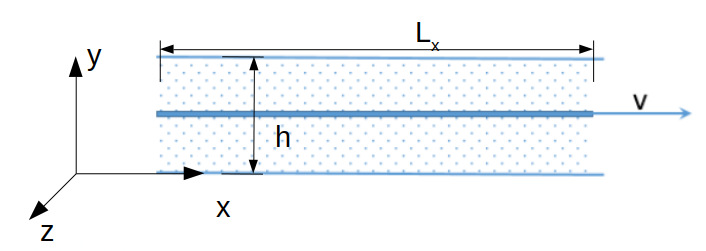
\includegraphics[width=0.5\linewidth]{plate.png}
   \end{center}
    \caption{\label{plate} Problem \ref{prb1} }
  \end{figure}


%====================================================================
\item {\bf Egyptian water clock:}
  An Egyptian water clock is a bowl with a small hole at the
  bottom. Time is measured by the fall of water level in this bowl as
  water flows out of the small hole in the bottom. To be able to
  function as a clock the rate of fall of the water level must be
  constant as a function of time for some interval of time.
  Wikipedia states: ``The oldest documentation of the water clock is
  the tomb  inscription
  of the 16th century BC Egyptian court official Amenemhet,
  which identifies himself as its inventor''. Let us see if you can
  design one. The bowl is a surface of revolution whose
  cross-section is shown in figure~\ref{fig:clock}.
  The surface is well-defined if we give the radius of the bowl, $R(H)$
  as a function of its height $H$.
  \begin{figure}[h]
    \begin{center}
      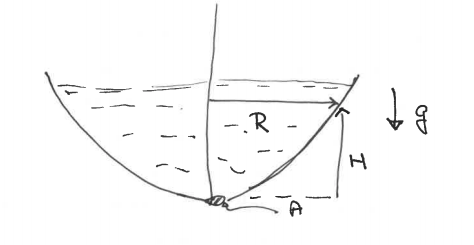
\includegraphics[width=0.5\linewidth]{egypt.png}
     \end{center}
    \label{fig:clock}
   \end{figure}
  \begin{enumerate}
\item At time $t$, let the height of the water in the bowl be
  $H(t)$. What is the velocity, $v(t)$, of the water flowing out of the hole at
  that instant?  Write clearly what assumptions you have made in
  arriving at the answer.
  \item If the area of the hole is $A$, the rate at which water flows
    out of the hole is $Q = v A C $ where $C$ is an empirically
    determined constant. In a small time $\Delta t$, the amount of
    water that flows out of this hole is given by $Q\Delta t$. If the
    fall in height in this small time interval is $\Delta H$, then
    \begin{equation}
      Q\Delta t = \pi R^2(H)\Delta H
      \end{equation}
    where $R$ is the radius of the bowl at the height $H$. To be able
    to function as a clock the rate of fall of $H$ must be a
    constant. Find $H$ as a function of $R$.
  \item If an ancient Egyptian brought this clock from Egypt to Sweden,
    would it work equally well? 
  \end{enumerate}

(8 p) \\  
  



  \end{enumerate}
%---------------------------------------------------------%


\end{document}
